% latex article template

% cheat sheet(eng): http://www.pvv.ntnu.no/~walle/latex/dokumentasjon/latexsheet.pdf
% cheat sheet2(eng): http://www.pvv.ntnu.no/~walle/latex/dokumentasjon/LaTeX-cheat-sheet.pdf
% reference manual(eng): http://ctan.uib.no/info/latex2e-help-texinfo/latex2e.html

% The document class defines the type of document. Presentation, article, letter, etc. 
\documentclass[12pt, a4paper]{article}

% packages to be used. needed to use images and such things. 
\usepackage[pdfborder=0 0 0]{hyperref}
\usepackage[utf8]{inputenc}
\usepackage[english]{babel}
\usepackage{graphicx}
\PassOptionsToPackage{hyphens}{url}

% hides the section numbering. 
\setcounter{secnumdepth}{-1}

% Graphics/image lications and extensions. 
\DeclareGraphicsExtensions{.pdf, .png, .jpg, .jpeg}
\graphicspath{{./images/}}

% Title or header for the document. 
\title{
	TIØ4116, Exercise 9. 
}
% Author
\author{
	Magnus L. Kirø \\
}
\date{\today}

\begin{document}
\maketitle
\pagenumbering{arabic}

\section{Task 1}
4 models

two parts:
1: cost=10 000 000 000
2: 500 000 per car. 

factory sales price = pf

mutual price across dealers. PK

demand = 300 000 - (PK /4)

dealer costs per car = 50 000
dealer operating costs 5 000 000 000

\paragraph{A}
pk=pf+50000
d=300000-(pk/4)
manufacturer cost, mc=10*10\^9 +500 000d
dealer cost, dc=5*10\^9 +50 000d
total cost, tc=15*10\^9 + 550000(300000-((pf+50000)/4))

Total cost is described by tc, where pf is
the price of a car from the manufacturer. 

The number of cars to sell in the value chain is found by solving the equation
above in regards to p when y=0. This minimizes the cost, and maximizes the
profit per car. This results in a car price of 1 259 090. And a total cost of
12500. Followed by solving dc given the now known pk. Which gives the number of
cars as: dc/(necessary profit per car)=(number of cars sold with dealer).
Assuming profit as 25 00 per car we get number of cars = 5. 

\paragraph{B}
Given the max of the demand function we get a demand of 12500. This is the
optimal number of cars to sell from the manufacturer. This results pk of 1.6*10\^6. 

\paragraph{C}
With cars sold=12500 we get the most created value in the value chain. Or
rather the lowest production costs, giving the most room for profit. 
The minimized costs happen at pf=1 150 000, and pk=1 200 000. 

\paragraph{D}
Porche could have maximized the manufacturer cost so that the profits would be
higher. 

\section{Task 2}
\paragraph{A}
p = price, 
demand = 100*10\^6 -(50*10\^3)p,
p = ((100*10\^6)-d)/50*10\^3,
tc = d(500 + pm + pi),
profit = p - tc,

This gives the profit graph as:
\begin{figure}[htb]
    \centering
    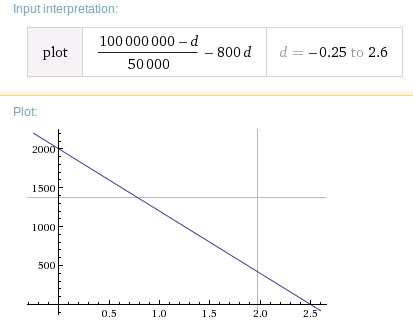
\includegraphics[width=\textwidth]{plot} 
    \label{plot}
    \caption{}
Plot for task 2a.
\end{figure}

Profit is maximized when demand goes towards 0. 

\paragraph{B}
pmi will be: ((100*10\^6)-d)/50*10\^3 -500, which is the total price minus the
price for assembly and other parts. 
\begin{figure}[htb]
    \centering
    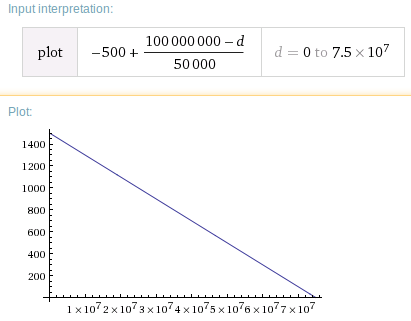
\includegraphics[width=\textwidth]{plot1}  
    \label{plot1}
    \caption{}
Plot for task 2b.
\end{figure}

\paragraph{C}
p = ((100*10\^6)-d)/50*10\^3,
Intel: pi=((100*10\^6)-d)/50*10\^3 -500-pm,
microsoft: pm=((100*10\^6)-d)/50*10\^3 -500-pi,

Contribution margin = price - variable cost.
Intel = p - pi,
microsoft = p -pm. 

A nash equilibrium is when the two parts don't benefit from changing position,
giving that both parties know the strategies of the other. 

\paragraph{D}
It is best for the consumers to have microsoft and intel to sell their products
individually. Microsoft and Intel will have a price advantage if they work in a
cartel. A cartel gives benefits to all parties in the cartel, and aims to
maximize profit for all parties. 

It would be quite easy for intel and microsoft to work together in a cartel
given subtask b.  

\section{Task 3}
\paragraph{A}
Assuming that q1 = q1 we get a set of two equations with two unknowns. Solving
this set we get q=24, p1=14, and p2=8. 
\begin{figure}[htb]
    \centering
    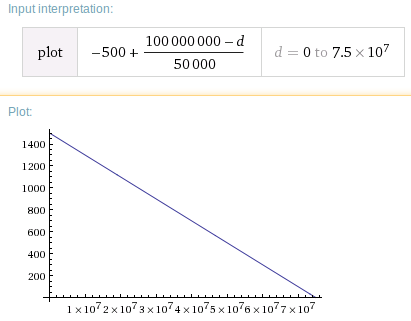
\includegraphics[width=\textwidth]{plot1}
    \label{plot1}
    \caption{}
Plot for task 3a.
\end{figure}

\paragraph{B}
q1 = coca cola
q2 = pepsi. 
\begin{figure}[htb]
    \centering
    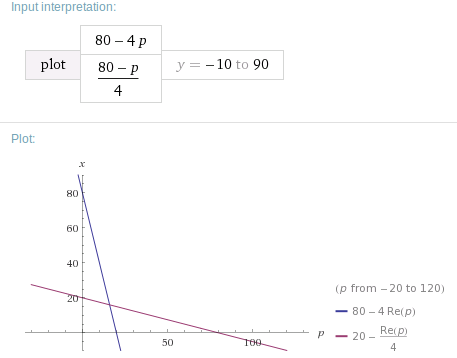
\includegraphics[width=\textwidth]{q1}
    \label{q1}
    \caption{}
task 3b, q1
\end{figure}

\begin{figure}[htb]
    \centering
    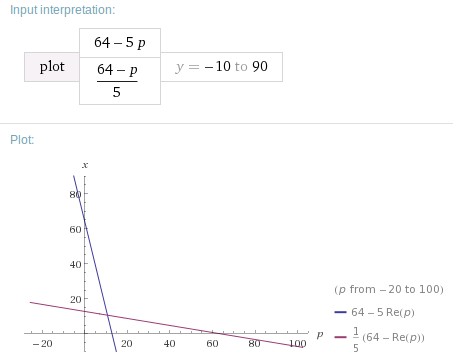
\includegraphics[width=\textwidth]{q2}
    \label{q2}
    \caption{}
task 3b, q2
\end{figure}

\paragraph{C}
Price elasticity: 

e=(\% change in demand)/(\% change in price),
e(coca cola)= (1/14) / (-9/24) = -0.2,
e(pepsi)= (3/11) / (-13/24) = -0.5,

\paragraph{D}
e = (\% Change in Quantity Demanded of Good X)/(\% Change in Price of Good Y), 
e = (1/14) / (-13/24) = -0.13, or e = (3/11) / (-9/14) = -0.42

\paragraph{E}
\begin{figure}[htb]
    \centering
    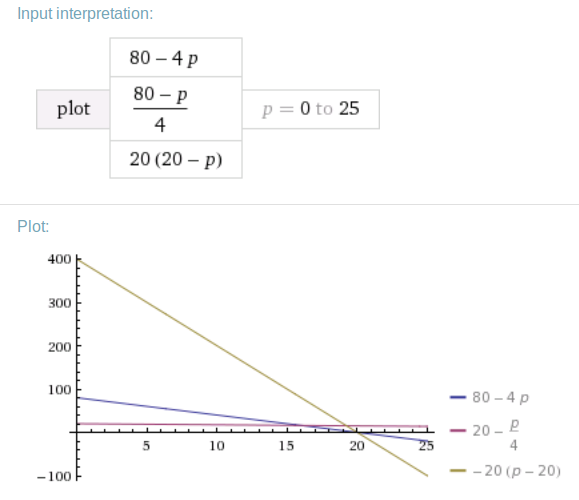
\includegraphics[width=\textwidth]{plot4}
    \label{plot4}
    \caption{}
task 3e
\end{figure}
From the graph we can see that the equilibrium mostly indicates surplus in
supply. If coca cola reduces costs the demand the price would go down and the
demand would go up. And we would balance the equilibrium more. 

\end{document}
This is never printed
